\documentclass[tikz,border=10pt]{standalone}
\begin{document}
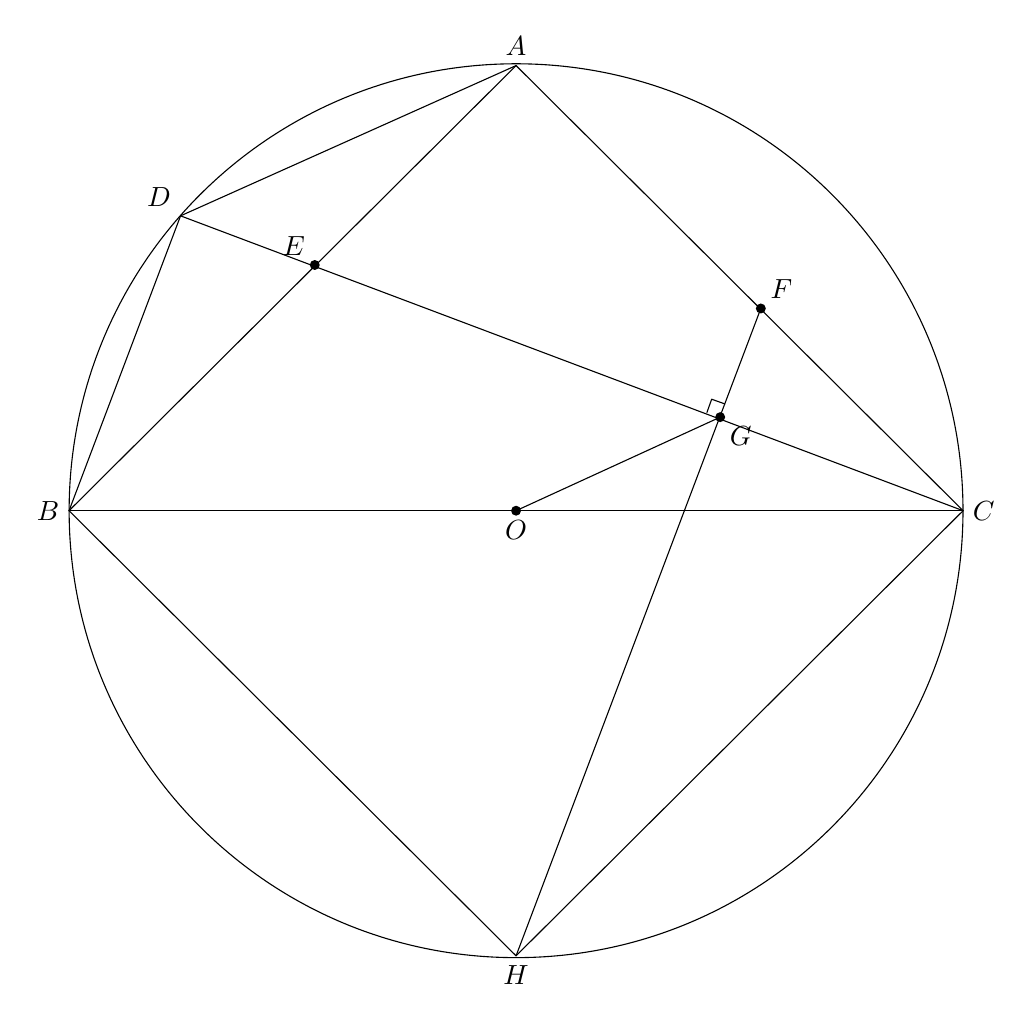
\begin{tikzpicture}[scale=1.2, line cap=round, line join=round]
  % Points
  \coordinate (O) at (0,0);
  \coordinate (A) at (0,4.71);
  \coordinate (B) at (-4.73,0);
  \coordinate (C) at (4.73,0);
  \coordinate (H) at (0,-4.71);
  \coordinate (D) at (-3.55,3.12);
  \coordinate (E) at (-2.13,2.60);
  \coordinate (F) at (2.59,2.14);
  \coordinate (G) at (2.16,0.99);

  % Circle
  \draw (O) circle (4.73);

  % Edges
  \draw (A) -- (D);
  \draw (D) -- (B);
  \draw (B) -- (A);
  \draw (A) -- (C);
  \draw (B) -- (H);
  \draw (H) -- (C);
  \draw (B) -- (C);
  \draw (D) -- (C);
  \draw (H) -- (F);
  \draw (O) -- (G);

  % Right angle mark at G
  \draw (2.21,1.13) -- (2.07,1.18) -- (2.02,1.04);

  % Points
  \fill (O) circle (1.5pt);
  \fill (E) circle (1.5pt);
  \fill (F) circle (1.5pt);
  \fill (G) circle (1.5pt);

  % Labels
  \node[above] at (A) {$A$};
  \node[left] at (B) {$B$};
  \node[right] at (C) {$C$};
  \node[below] at (H) {$H$};
  \node[above left] at (D) {$D$};
  \node[above left] at (E) {$E$};
  \node[above right] at (F) {$F$};
  \node[below right] at (G) {$G$};
  \node[below] at (O) {$O$};
\end{tikzpicture}
\end{document}
